%%%% Proceedings format for most of ACM conferences (with the exceptions listed below) and all ICPS volumes.
\documentclass[sigconf]{acmart}
%%%% As of March 2017, [siggraph] is no longer used. Please use sigconf (above) for SIGGRAPH conferences.

%%%% Proceedings format for SIGPLAN conferences 
% \documentclass[sigplan, anonymous, review]{acmart}

%%%% Proceedings format for SIGCHI conferences
% \documentclass[sigchi, review]{acmart}

%%%% To use the SIGCHI extended abstract template, please visit
% https://www.overleaf.com/read/zzzfqvkmrfzn

\usepackage{booktabs} % For formal tables
\usepackage{tikz}     % For drawing example boxes
\usepackage{graphicx}
\usetikzlibrary{positioning}

% Copyright
\setcopyright{none}
%% \setcopyright{acmcopyright}
%\setcopyright{acmlicensed}
%%\setcopyright{rightsretained}
%\setcopyright{usgov}
%\setcopyright{usgovmixed}
%\setcopyright{cagov}
%\setcopyright{cagovmixed}


% DOI
% \acmDOI{}

% ISBN
% \acmISBN{}

%Conference
% \acmConference[WOODSTOCK'97]{ACM Woodstock conference}{July 1997}{El Paso, Texas USA} 
% \acmConference[ACMSE 2018]{ACM Southeastern conference}{March 2018}{Richmond, Kentucky USA} 
% \acmYear{2018}
% \copyrightyear{2018}

% \acmArticle{4}
% \acmPrice{0.00}

% These commands are optional
%\acmBooktitle{Transactions of the ACM Woodstock conference}
%\editor{Jennifer B. Sartor}


\begin{document}
\title{Novel Meshes for Multivariate Interpolation and Approximation}
%\titlenote{Produces the permission block, and copyright information}
%\subtitle{Extended Abstract}
%\subtitlenote{The full version of the author's guide is available as \texttt{acmart.pdf} document}

%% \author{Thomas C. H. Lux}
%% %\authornote{Dr.~Trovato insisted his name be first.}
%% %\orcid{1234-5678-9012}
%% \affiliation{%
%%   \institution{Virginia Polytechnic and State University}
%% %  \streetaddress{P.O. Box 1212}
%%   \city{Blacksburg} 
%%   \state{Virginia} 
%%   \postcode{24060}
%% }
%% \email{tchlux@vt.edu}

%% \author{Layne Watson}
%% %\authornote{Dr.~Trovato insisted his name be first.}
%% %\orcid{1234-5678-9012}
%% \affiliation{%
%%   \institution{Virginia Polytechnic and State University}
%% }

%% \author{Tyler H. Chang}
%% %\authornote{Dr.~Trovato insisted his name be first.}
%% %\orcid{1234-5678-9012}
%% \affiliation{%
%%   \institution{Virginia Polytechnic and State University}
%% }

%% % The default list of authors is too long for headers.
%% \renewcommand{\shortauthors}{T. Lux et al.}


\begin{abstract}

A rapid increase in the quantity of data available is allowing all fields of science to generate more accurate models of multivariate phenomena. Regression and interpolation become challenging when the dimension of data is large, especially while maintaining tractable computational complexity. This paper proposes three novel techniques for multivariate interpolation and regression that each have polynomial complexity with respect to number of instances (points) and number of attributes (dimension). Initial results suggest that these techniques are capable of effectively modeling multivariate phenomena while maintaining flexibility in different application domains.

\end{abstract}

%
% The code below should be generated by the tool at
% http://dl.acm.org/ccs.cfm
% Please copy and paste the code instead of the example below. 
%
% \begin{CCSXML}
% <ccs2012>
%  <concept>
%   <concept_id>10010520.10010553.10010562</concept_id>
%   <concept_desc>Computer systems organization~Embedded systems</concept_desc>
%   <concept_significance>500</concept_significance>
%  </concept>
%  <concept>
%   <concept_id>10010520.10010575.10010755</concept_id>
%   <concept_desc>Computer systems organization~Redundancy</concept_desc>
%   <concept_significance>300</concept_significance>
%  </concept>
%  <concept>
%   <concept_id>10010520.10010553.10010554</concept_id>
%   <concept_desc>Computer systems organization~Robotics</concept_desc>
%   <concept_significance>100</concept_significance>
%  </concept>
%  <concept>
%   <concept_id>10003033.10003083.10003095</concept_id>
%   <concept_desc>Networks~Network reliability</concept_desc>
%   <concept_significance>100</concept_significance>
%  </concept>
% </ccs2012>  
% \end{CCSXML}

% \ccsdesc[500]{Computer systems organization~Embedded systems}
% \ccsdesc[300]{Computer systems organization~Redundancy}
% \ccsdesc{Computer systems organization~Robotics}
% \ccsdesc[100]{Networks~Network reliability}

\keywords{Interpolation, Approximation, Splines, Multivariate, Regression}

\maketitle

\section{Introduction}
\label{sec_introduction}

Regression and interpolation are problems of considerable importance that find applications across many fields of science. Pollution and air quality analysis \cite{de2008field}, energy consumption management \cite{lazos2014optimisation}, and student performance prediction \cite{cortez2008using} are a few examples of interdisciplinary applications of multivariate regression for predictive analysis. As discussed later, these techniques can also be applied to prediction problems related to high performance computing (HPC) file input/output (I/O), Parkinson's patient clinical evaluations \cite{tsanas2010accurate}, and forest fire risk assessment \cite{cortez2007data}.

Multivariate interpolation is formally defined when there exists some function $f:\mathbb{R}^d \rightarrow \mathbb{R}$ and a set $X$ of $n$ points in $\mathbb{R}^d$ along with associated response values $f(x)$ for all $x \in X$. The problem is to construct an approximation $\hat f: \mathbb{R}^d \rightarrow \mathbb{R}$ such that $\hat f(x) = f(x)$ for all $x \in X$. It is often the case that the form of the true underlying function $f$ is unknown, however it is still desirable to construct an approximation $\hat f$ with minimum approximation error at $y \notin X$.

Multivariate regression is often used when the underlying function is presumed to be stochastic, or stochastic error is introduced in the evaluation of $f$. Hence, multivariate regression relaxes the conditions of interpolation by minimizing the error in $\hat f$ at $x \in X$ while maintaining some parametric form with parameters $P$. This can be written as $\min_{P} ||\hat f(X) - f(X)||$, where $f(X)$ is a vector of $f(x)$ for all $x \in X$ and $||\cdot||$ is an appropriate measure. The difficult question in the case of regression is often what parametric form to adopt for any given application. This paper proposes basis functions with overlapping regions of support as the general parametric form.

As the dimension of data increases, the number of possible interactions between dimensions grows exponentially. Quantifying all possible interactions becomes intractable and hence beyond three-dimensional data, mostly linear models are used. That is not to say nonlinear models are absent, but nonlinearities are often either preconceived or model pairwise interactions between dimensions at most. Similarly, higher order models of single variables can be generated from the techniques proposed in this paper, however only first-order interactions between variables are considered.

Regression and interpolation have a considerable theoretical base in one dimension \cite{cheney2009course}. Splines in particular are well understood as an interpolation technique in one dimension \cite{de1978practical}, particularly B-splines. Fewer techniques have been discussed and evaluated for two dimensional problems. Though in two and three dimensions tensor product splines remain computable \cite{unther1996interpolating}, tensor products have an unfortunate exponential scaling in parameterization with increasing dimension. Exponential scaling prohibits tensor products from being reasonably applied beyond three-dimensional data. In order to address this dimensional scaling challenge, C. de Boor and others have recently proposed box splines \cite{de2013box}. Two of the three meshes introduced in this work involve box-shaped regions of support and use box splines as the underlying basis functions.

% Art is a subjective form of personal expression and computers are just robots that are going to take over the world. \textit{*deep breath*} In order to communicate my frustration with the technological and information revolution, I'm going to write the rest of this paper in poetry.

% Star light, star bright \ldots

\subsection{Box Splines}
\label{sec_box_splines}

\begin{figure}
  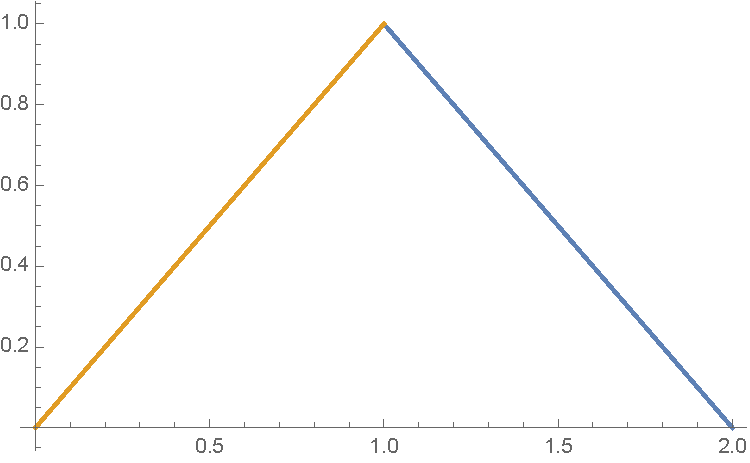
\includegraphics[width=0.23\textwidth,height=2.5cm]{1D-linear.pdf}
  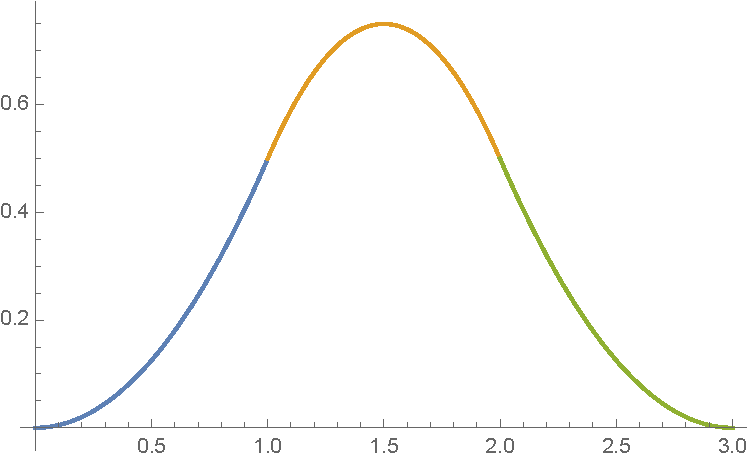
\includegraphics[width=0.23\textwidth,height=2.5cm]{1D-quadratic.pdf}
  \caption{1D linear (order 2) and quadratic (order 3) box splines with direction vector sets $\bigl( 1 \ 1 \bigr)$ and $\bigl( 1 \ 1 \ 1 \bigr)$ respectively. Notice that these direction vector sets form the B-Spline analogues, order 2 composed of two linear components and order 3 composed of 3 quadratic components (colored in plot).
  \vspace{-.5cm}}
  \label{fig_1D_boxes}
\end{figure}

A box spline in $\mathbb{R}^d$ is defined by its \textit{direction vector set} $A$, composed of $s$ $d$-vectors where $s \geq d$. Further, $A$ will be written as a $d \times s$ matrix. The first $m$ column vectors of $A$ are denoted by $A_m$, $m \leq s$. $A_d$ is required to be nonsingular. Consider the unit cube in $s$ dimensions $Q_s = [0,1)^s$. $A_s \bigl( Q_s \bigr)$ is now the image (in $d$ dimensions) of $Q_s$ under the linear map $A$. This image is the region of support for the box spline defined by $A_s$ in $d$ dimensions. The box spline function in $d$ dimensions for $A_d$ is defined as
\begin{equation}
B(x \mid A_d) = \begin{cases} 
(\det(A_d))^{-1}, & x \in A_d(Q_d), \\
0,                & \text{otherwise.}
\end{cases}
\label{eq_box_base}
\end{equation}
For $A_s$ when $s > d$ the box spline is computed as
\begin{equation}
B(x \mid A_s) = \int_0^1 B(x - t v_s \mid A_{s-1}) dt,
\label{eq_box_recursive}
\end{equation}
where $v_s$ is the $s$th direction vector of $A$.

The application of box splines presented in this paper always utilizes the $d$-dimensional identity matrix as $A_d$. This simplifies the computation in Equation \ref{eq_box_base} to be the indicator function over the unit cube. Composing $A$ strictly out of $k$ repetitions of the identity matrix forms the $k$th order B-spline with knots located at $0$, $1$, $\ldots$, $k-1$, $k$ along each axis (see Figure \ref{fig_1D_boxes}). Furthermore, while the number of subregions for the $k$th order $d$-dimensional box spline grows as $k^d$ (see Figure \ref{fig_2D_boxes}), the symmetry provided by direction vector sets composed of repeated identity matrices allows the computation of box splines to be simplified. The value of a box spline at any location is then the product of all axis-aligned 1-dimensional $k$th order box splines.

The box splines as presented are viable basis functions. Each box spline can be shifted and scaled without modifying the underlying computation (similar to wavelets), yet the underlying computation is simple and scales linearly with dimension. For a more thorough introduction and exploration of box splines in their more general form, readers are referred to \cite{de2013box}. 

\begin{figure}
  \vspace{-.5cm}
  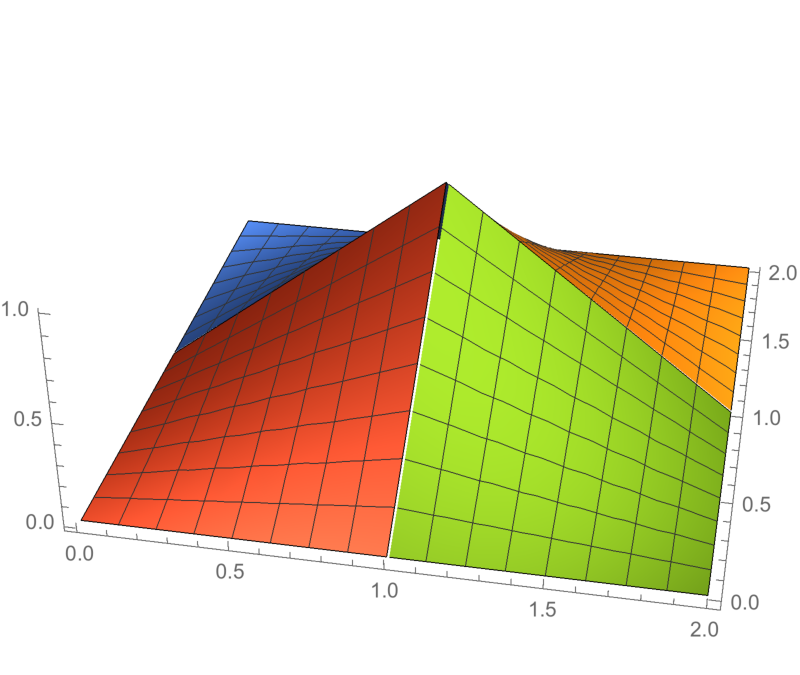
\includegraphics[width=0.23\textwidth,height=3cm]{2D-linear.pdf}
  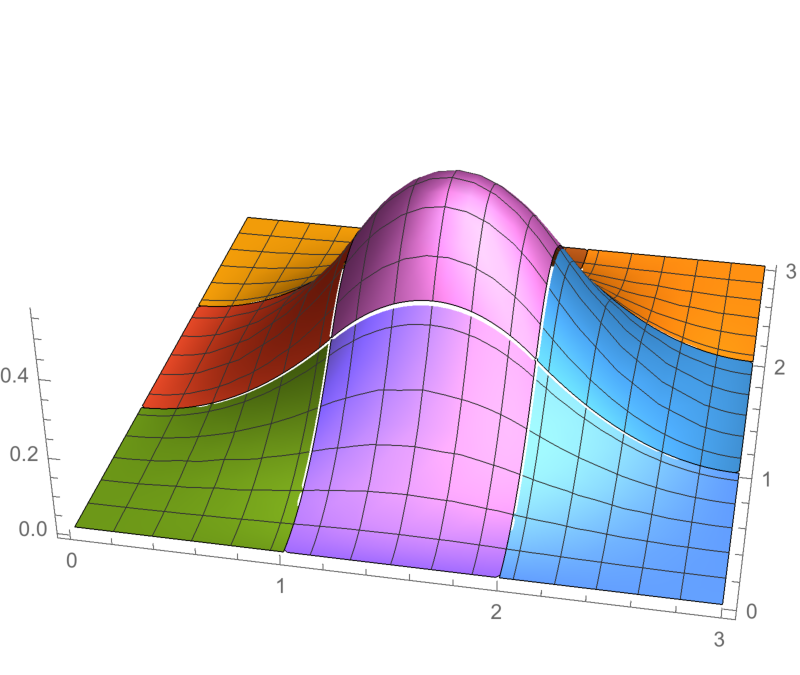
\includegraphics[width=0.23\textwidth,height=3cm]{2D-quadratic.pdf}
  \caption{2D linear (order 2) and quadratic (order 3) box splines with direction vector sets $\bigl( I \ I \bigr)$ and $\bigl( I \ I \ I \bigr)$ respectively, where $I$ is the identity matrix in two dimensions. Notice that these direction vector sets also produce boxes with $\text{order}^2$ subregions (colored in plot).
  \vspace{-0.1cm}}
  \label{fig_2D_boxes}
\end{figure}

\section{Interpolation and Regression}
\label{sec_mesh_construction}

Throughout this section, the same notation will be used as introduced in Section \ref{sec_introduction}. $X \subset \mathbb{R}^d$ is a finite set of points with known response values $f(x)$ for all $x \in X$.

Define a box $b^c = (c,l^c,u^c)$ in $d$ dimensions with center $c \in \mathbb{R}^d$, lower width vector $l^c \in \mathbb{R}^d_+$, and upper width vector $u^c \in \mathbb{R}^d_+$ (where $u^c_i$ refers to the $i$th component of $u^c$). A visual example of a box in two dimensions can be seen in Figure \ref{fig_example_box}. Now, define a componentwise rescaling function $g: \mathbb{R}^d \rightarrow \mathbb{R}^d$ at point $x \in \mathbb{R}^d$ to be
\begin{equation}
  \bigl(g^c(x)\bigr)_r = {k \over 2} \left( 1 + {(x_r - c_r)_- \over l^c_r} - {(x_r - c_r)_+ \over u^c_r} \right)
\end{equation}
where $y_+=\max\{y,0\}$, $y_-=(-y)_+$, $k$ is the order of the box spline as described in Section \ref{sec_box_splines}. Finally, each box spline in a box mesh can be evaluated as $B(g^c(x) \mid A)$ presuming the order of approximation implies $A$. Both box meshes described in the following subsections use box spline basis functions of this form.

A notable property of boxes defined with the linear rescaling function $g^c$, is that $C^0$ and $C^1$ continuity of the underlying box spline are maintained. $C^0$ continuity is maintained through scaling. $C^1$ continuity is maintained for all box splines with $C^1$ continuity (order $\geq 3$) because the scaling discontinuity is located at $c$, where all box splines (of the presented form) have first derivative zero. All continuity beyond the first derivative is lost through the rescaling function $g^c$.

\begin{figure}
  \centering
  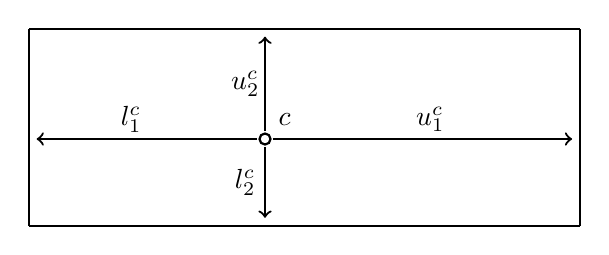
\begin{tikzpicture}[scale=1]
    \draw[thick] (3,1.1) circle (0.7mm);

    %% Draw arrows for each width
    \draw[thick,->] (3,1.2) -- (3,2.4);
    \draw[thick,->] (3,1.0) -- (3,0.1);
    \draw[thick,->] (3.1,1.1) -- (6.9,1.1);
    \draw[thick,->] (2.9,1.1) -- (0.1,1.1);

    %% Draw boundary of box
    \draw[thick,-] (0,0) -- (7,0);
    \draw[thick,-] (7,0) -- (7,2.5);
    \draw[thick,-] (7,2.5) -- (0,2.5);
    \draw[thick,-] (0,2.5) -- (0,0);

    %% Add text to the picture
    \node at (3.25,1.35) {$c$};
    \node at (1.3,1.35) {$l^c_1$};
    \node at (5.1,1.35) {$u^c_1$};
    \node at (2.75,0.55) {$l^c_2$};
    \node at (2.75,1.8) {$u^c_2$};
  \end{tikzpicture}
  \caption{An example box in two dimensions with center $c$, upper widths $u^c_1$, $u^c_2$, and lower widths $l^c_1$, $l^c_2$. Notice that $c$ is not required to be equidistant from opposing sides of the box, that is $u^c_i \not= l^c_i$ is allowed.}
  \label{fig_example_box}
\end{figure}

\subsection{Max Box Mesh}

The first of the three meshes produces a set of boxes around chosen control points and each box has maximal distance between the control point and the nearest side of the box. This centrality property is one mechanism of creating the largest reasonable regions of support for the underlying basis functions. The individual boxes are constructed via the following procedure given a set of control points $C \subseteq X$, $c^{(i)} \in C$,
\begin{enumerate}
  \item Initialize a box $b^{c^{(1)}} \supset X$ with center $c^{(1)}$. \label{step_init}
  \item Identify $c^{(i)}$ over $\bigl\{ j \bigm| j \ne 1$, $B^{c^{(1)}}\bigl( c^{(j)} \bigr) \ne 0 \bigr\}$ that minimizes $\bigl\|c^{(j)}-c^{(1)}\bigr\|_\infty$.  \label{step_closest}
  \item Change the the box $b^{c^{(1)}}$ along the first dimension $r$ such that $\bigl|\bigl|c^{(1)} - c^{(i)}\bigr|\bigr|_\infty = \bigl\vert c^{(1)} - c^{(i)}\bigr\vert_r $, to exclude $c^{(i)}$ from the support of $B^{c^{(1)}}$. \label{step_shrink}
  \item Repeat steps \ref{step_closest} and \ref{step_shrink} until no point in $C$ is in the support of $B^{c^{(1)}}$ (at most $2d$ times, once for each boundary of a box).
\end{enumerate}

The same process is used to construct boxes around all control points in $C$. In order to improve the generality of the approximation, a set of control points is initially chosen to be well-spaced using a statistical method from \cite{amos2014algorithm}:

\begin{enumerate}
\item Generate a sequence of all pairs of points sorted by ascending pairwise Euclidean distance between points $\bigl(x^{(i_1)},x^{(j_1)}\bigr)$, $\bigl(x^{(i_2)},x^{(j_2)}\bigr)$, $\ldots$ , so that $\bigl\|x^{(i_k)}-x^{(j_k)}\bigr\|_2 \leq \bigl\|x^{(i_{k+1})}-x^{(j_{k+1})}\bigr\|_2$.
\item Sequentially remove points from candidacy until only $|C|$ remain by randomly selecting a single point from each pair $\bigl(x^{(i_m)}, x^{(j_m)}\bigr)$ for $m = 1,\ldots$ if both $x^{(i_m)}$ and $x^{(j_m)}$ are still candidates for removal.
\end{enumerate}

Once the boxes for a max box mesh have been constructed, the parameters can be identified via a least squares fit. The max box mesh (denoted $MBM$) is used to generate a $|X| \times |C|$ matrix $M$ of box spline basis function evaluations at all points in $X$. The solution to the least squares problem $\min_P \bigl\| M \ P - f(X) \bigr\|_2$ is the parameterization of $MBM$. When $C = X$, $M$ is the $|X| \times |X|$ identity matrix, making the max box mesh approximation $\hat f$ an interpolant.

While setting the number of boxes equal to the number of points causes the max box mesh to be an interpolant, the generality of the max box mesh approximation can often be improved by bootstrapping the selection of control points. Given a user-selected batch size $s \leq |X|$, start with $s$ well-spaced control points. Next, measure the approximation error at $x \notin C$ and if the error is too large (determined by user), pick $s$ points at which the magnitude of approximation error is largest, add those points to $C$, and recompute the max box mesh. The user is left to decide the batch size $s$ and the error tolerance based on validation performance and computability. Next, the max box mesh is shown to be nearly space filling.


\begin{definition}
A box $b^y$ is the upper \textit{boundary} of box $b^x$ along dimension $r$ if and only if $u^x_r = (y_r - x_r)$. A box $b^y$ is the lower \textit{boundary} of box $b^x$ along dimension $r$ if and only if $l^x_r = (x_r - y_r)$.
\end{definition}

\begin{definition}
A \textit{proper} upper boundary for box $b^x$ at point $y$ occurs when $u^x_r = ||x - y||_\infty$ and $r$ is the first dimension such that $u^x_r = ||x - y||_\infty$, assuming dimensions are deterministically ordered. The same definition applies to lower boundaries.
\end{definition}

\begin{theorem}
A max box mesh composed of $n$ unique control points in $d$ dimensions, $C \subset \mathbb{R}^d$ where all boundaries are proper, is nearly space filling.
\label{theorem_mutual_space_filling}
\end{theorem}
\begin{proof}
Pick an arbitrary point $x \in \mathbb{R}^d$. Now let $c^{(1)}$ be the $c \in C$ that minimizes $|| c - x ||_\infty$, making the nearest box (by max norm) $b^{c^{(1)}}$. Either $x$ is in the support of $b^{c^{(1)}}$ or on the boundary of $b^{c^{(1)}}$ and this is done, or $b^{c^{(1)}}$ has a proper boundary along dimension $r$ with box $b^{c^{(2)}}$ such that $|c^{(2)}_r - x_r| < |c^{(1)}_r - x_r|$. The sequence of bounds $c^{(2)}$, $\ldots$, must be finite for the strict inequality to hold and the last box in this sequence supports $x$. Therefore, the $MBM$ is nearly space filling.
\end{proof}

The max box mesh as proposed is still capable of producing coefficients of 0 for $x \in \mathbb{R}^d$ placed along the boundary of boxes, however this problem is solved by increasing the upper and lower widths of all boxes by the unit roundoff during computation. For this reason, the max box mesh remains a viable strategy for computed approximations. Given a maximum of $c$ control points in $d$ dimensions with $n$ points, the computational complexities are: $\mathcal{O}(c^2 d)$ for computing boxes, $\mathcal{O}(c d^2 + d^3)$ for a least squares fit, and $\mathcal{O}(n / s)$ for bootstrapping (which is multiplicative over the fitting complexities). Evaluating the max box mesh requires $\mathcal{O}(c d)$ computations.

\subsection{Iterative Box Mesh}

The iterative box mesh ($IBM$) composes box-shaped regions of support over control points that each support strictly one control point just as in the $MBM$, however the mesh is completely space filling by construction and places boxes in a way that reduces apparent error. The boxes are constructed via the following procedure given a finite set of points $X \subset \mathbb{R}^d$,
\begin{enumerate}
\item Add a box with total support around the most central point $x^{(1)} \in X$ to $IBM$ and fit the mesh to all $X$.
\item Add a box centered at $x^{(i)} \notin IBM$ that has the most approximation error, reshaping all boxes in $b^{x^{(j)}} \in IBM$ that contain $x^{(i)}$ by bounding the first dimension $r$ such that $\bigl| x^{(j)}_r - x^{(i)}_r \bigr| = \bigl| \bigl| x^{(j)} - x^{(i)} \bigr| \bigr|_\infty$ and then fit the mesh to all $X$. \label{step_add_box}
\item Repeat Step \ref{step_add_box} until approximation error is below tolerance $t$.
\end{enumerate}

Just as the $MBM$, the parameters can be identified via a least squares solve. The iterative box mesh is used to generate a $|X| \times |C|$ matrix $M$ of box spline function evaluations at all points in $X$. Now the set of coefficients for each box is the solution to the least squares problem $\min_P \bigl|\bigl| M\ P - f(X) \bigr|\bigr|_2$. Also as for the $MBM$, $C = X$ causes $M$ to equal the $|X| \times |X|$ identity, making the iterative box mesh approximation $\hat f$ an interpolant.

As opposed to the max box mesh, the bootstrapping procedure is built into the iterative box mesh. The user is left to decide the most appropriate error tolerance, however a decision mechanism and analysis is presented in Section \ref{sec_performance_analysis}. Next, it is shown that the $IBM$ is space filling.

\begin{definition}
A \textit{mutual} boundary between boxes $b^x$ and $b^y$ is when there exists an $r$ such that $u^x_r = l^y_r$ or $l^x_r = u^y_r$.
\end{definition}

\begin{theorem} An iterative box mesh composed of $n$ unique control points in $d$ dimensions, $C \subset \mathbb{R}^d$, is space filling. \end{theorem}
\begin{proof}
The first box added to an $IBM$ is space filling by construction. Assume that an $IBM$ composed of $n$ boxes is space filling and a new box centered at $x \in \mathbb{R}^d$ is added. Consider a point $y \in \mathbb{R}^d$. Every box $b^{x^{(i)}}$ that supported $y$ before the addition of $b^x$ and was reshaped along dimension $r \in [1,d]$ has a mutual boundary with $b^x$ by construction. Now either $\bigl| x_r - x^{(i)}_r \bigr| \geq \bigl| y_r - x^{(i)}_r \bigr|$ and $b^{x^{(i)}}$ still supports $y$, or $\bigl| x_r - x^{(i)}_r \bigr| < \bigl| y_r - x^{(i)}_r \bigr|$ and $b^x$ supports $y$. Therefore, the $IBM$ composed of $n+1$ boxes is still space filling.
\end{proof}

After fitting for parameters, an $IBM$ can generate approximations for a set of new points $Z \subset \mathbb{R}^d$ by evaluating all box basis functions multiplied by the coefficients, $P$. The computational complexity for generating the mesh is $\mathcal{O}(c^2 n d)$ where $c$ is the number of control points determined by the minimum error threshold and $n = |X|$. The computational complexity of evaluating the mesh at a singple point is $\mathcal{O}(c d)$.

\subsection{Voronoi Mesh}

The final of the three meshes utilizes $\ell2$ norm distances to define boundaries rather than max norm distances. A well-studied technique for classification and approximation is the nearest neighbor algorithm \cite{cover1967nearest}. The convex region surrounding a central control point in which all points are closer to that center than any other control point is also called the Voronoi cell \cite{dirichlet1850reduction}. The Voronoi mesh ($VM$) utilizes Voronoi cells to define support via a generic basis function $v: \mathbb{R}^d \rightarrow \mathbb{R}$ with

\begin{equation}
v^c(z) = \left(1 - \frac{||z - c||_2}{2 \ dist(z - c \mid c)} \right)_+
\label{eq_voronoi_basis}
\end{equation}

where $c \in \mathbb{R}^d$ is the center of the Voronoi cell, $z \in \mathbb{R}^d$ is an interpolation point, and $dist(\ \cdot \mid c)$ is the distance between $c$ and the nearest boundary of the cell along the vector $\cdot\ $. While all basis functions $v^c(c) = 1$, the $2$ in the denominator causes all basis functions to go linearly to $0$ at the boundary of the twice-expanded Voronoi cell. Note that this basis function is $C^0$ because the boundaries of the Voronoi cell are $C^0$. In the case that there is no boundary along the vector $x-c$, the basis function value is always $1$.

While the cost of computing all Voronoi cells for any given set of points grows exponentially \cite{dutour2009complexity}, the calculation of $dist$ is linear with respect to the number of control points and dimensions. Given any center $c^{(1)} \in \mathbb{R}^d$, set of control points $C \subset \mathbb{R}^d$, and interpolation point $z \in \mathbb{R}^d$, $dist\bigl((z-c^{(1)}) \mid c^{(1)}\bigr)$ is the solution to
\begin{equation}
  \max_{\{c \in C\}\backslash c^{(1)}} \frac{|z|}{2} \ \frac{z \cdot \bigl(c - c^{(1)}\bigr) - c^{(1)} \cdot \bigl(c - c^{(1)}\bigr)}{c \cdot \bigl(c - c^{(1)}\bigr) - c^{(1)} \cdot \bigl(c - c^{(1)}\bigr)}.
\end{equation}

The parameters of the $VM$ can now be computed exactly as for the $MBM$ and $IBM$. The vornonoi mesh is used to generate a $|X| \times |C|$ matrix $M$ of basis function evaluations at all points in $X$. Now the set of coefficients for each basis function is the solution to the least squares problem $\min_P \bigl\| M \ P - f(X) \bigr\|_2$. When $X = C$, $M$ is the identity making the mesh an interpolant. Bootstrapping can be performed with an identical procedure to that of the $IBM$.
\begin{enumerate}
\item Pick the most central point $x^{(1)} \in X$ to be the first control point in $VM$ and fit the mesh to all $X$.
\item Add a control point $x^{(i)} \notin VM$ that has the most approximation error and then fit the mesh to all $X$. \label{step_add_control}
\item Repeat Step \ref{step_add_control} until approximation error is below tolerance $t$.
\end{enumerate}

Any $VM$ is na\"{\i}vely space filling, since any possible interpolation point will have a nearest neighbor control point when the set of control points is nonempty.

\begin{theorem}
  A Voronoi mesh composed of $n$ unique control points in $d$ dimensions, $C \subset \mathbb{R}^d$, is space filling.
\end{theorem}
\begin{proof}
  Consider interpolating at point $z$. Let $c^{(1)}$ be the $c \in C$ that minimizes $||z-c||_2$. Now, $z$ must be in the support of the basis function $v^{c^{(1)}}$. Therefore the Voronoi mesh is space filling.
\end{proof}

The computational complexity of evaluating a parameterized Voronoi mesh with $c$ control points is $\mathcal{O}(c^2 d)$. Bootrsapping the generation of a Voronoi mesh requres $\mathcal{O}(c^2 n d)$ computations for a maximum number of basis functions $c$ determined by the error threshold.

% \subsection{Boxed Natural Neighbor}
% \begin{itemize}
% \item How the mesh is generated
% \item How interpolation is done
% \end{itemize}

\section{Data and Analysis}
In order to evaluate the proposed interpolation and approximation techniques, this paper utilizes three data sets of varying dimension and application. In the following subsections the sources and targets of each data set are described, as well as challenges and limitations related to doing interpolation and approximation on these data sets. The distributions of response values being modeled can be seen in Figure \ref{fig_response_hists}. The preprocessing and approximation processes are described in Section \ref{sec_performance_analysis}.

\begin{figure}
  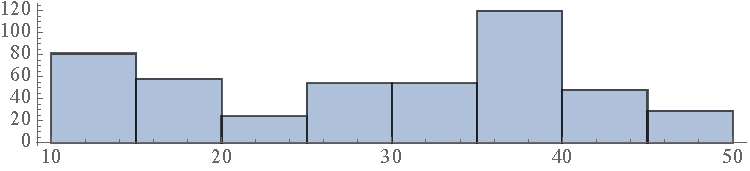
\includegraphics[width=.5\textwidth,height=2cm]{p-hist.pdf}
  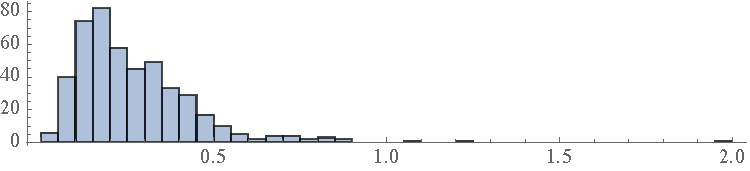
\includegraphics[width=.5\textwidth,height=2cm]{f-hist.pdf}
  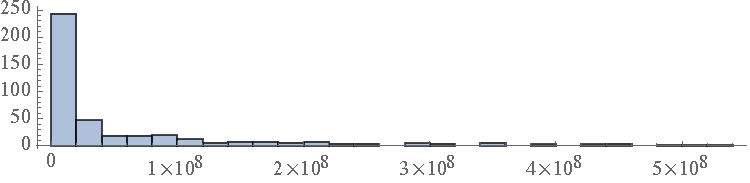
\includegraphics[width=.5\textwidth,height=2cm]{h-hist.pdf}
  \caption{Histograms of Parkinsons (total UPDRS), forest fire (area), and HPC I/O (mean throughput) response values respectively. Notice that both the forest fire and HPC I/O data sets are heavily skewed.
  \vspace{-.5cm}}
  \label{fig_response_hists}
\end{figure}

\subsection{Data Summary}

\subsubsection{High Performance Computing I/O}
$$N = 532, D = 4$$
The first of three data sets is a four-dimensional dataset produced by executing the IOzone benchmark from \cite{iozone} on a homogeneous cluster of computers. The system performance data was collected by executing IOzone 40 times for each of a select set of system configurations. A single IOzone execution reports the max I/O file-read throughput seen. The 40 executions for each system configuration are converted to their mean, which is capable of being modeled by each of the multivariate approximation techniques presented in Section \ref{sec_mesh_construction}. The four dimensions being modelled to predict throughput mean are file size, record size, thread count, frequency.

\subsubsection{Forest Fire}
$$N = 517, D = 12$$

The forest fire data set provided by \cite{cortez2007data}, describes the area of Montesinho park burned on specific days and months of the year in terms of the environmental conditions. The twelve dimensions being used to model burn area are the $x$ and $y$ spatial coordinates of burns in the park, month and day of year, the FFMC, DMC, DC, and ISI indices (see source for details), the temperature in celcius, relative humidity, wind speed, and outdoor rain. The original analysis of this data set demonstrated it to be difficult to model, likely due to the skew in response values.

\subsubsection{Parkinson's Telemonitoring}
$$N = 468, D = 16$$

The final data set for evaluation is derived from a speech monitoring study with the intent to automatically estimate Parkinson's disease symptom development in parkinsons patients from \cite{tsanas2010accurate}. Particularly, a time-consuming clincal evaluation measure referred to as the UPDRS score. The total UPDRS score given by a clinical evaluation is estimated through 16 real numbers generated from biomedical voice measures of in-home sound recordings.

\subsection{Performance Analysis}
\label{sec_performance_analysis}

\begin{figure*}[htb]
  \begin{tikzpicture}
    \node (img)  {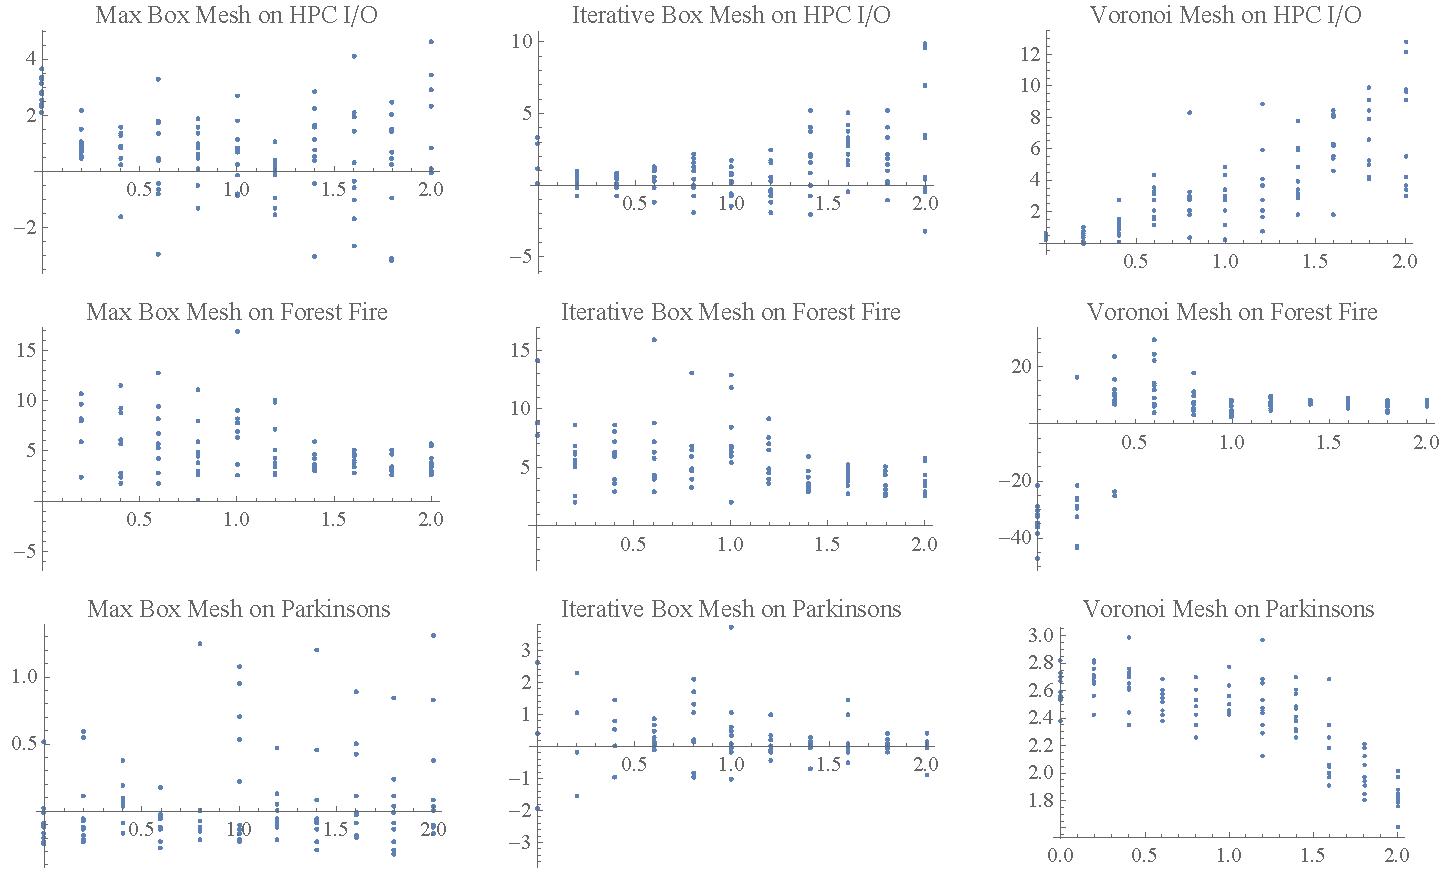
\includegraphics[width=0.95\textwidth,height=9.5cm]{all-performance.pdf}};
    \node[below=of img, node distance=0cm, yshift=1cm] {Relative Error Tolerance while Bootstrapping};
    \node[left=of img, node distance=0cm, rotate=90, anchor=center,yshift=-0.7cm] {Signed Relative Error};
  \end{tikzpicture}
  \caption{The performance of all three techniques with varied relative error tolerance for the bootstrapping parameter. The columns are for Max Box Mesh, Iterative Box Mesh, and Voronoi Mesh, respectively. The rows are for HPC I/O, Forest Fire, and Parkinsons respectively. Notice that the techniques exibit counterintuitive behavior on the Parkinsons and Forest Fire data sets, performance increases with increasing error tolerance.}
  \label{fig_all_performance}
\end{figure*}

The performance of the approximation techniques varies considerably across the three evaluation data sets. Relative errors for the most na\"{\i}ve approximators such as nearest neighbor can range $\displaystyle [0, \big(\max_x f(x) - \min_x f(x)\big) / \min_x f(x) ]$ when modeling a nonnegative function $f(x)$ from data. Each of the approximation techniques presented remain within these bounds and all errors are presented in signed relative form $(\hat f(x) - f(x)) / f(x)$. Before the models are constructed all data $X$ values are shifted and scaled to be in the unit cube $[0,1]$, while the response values are taken in their original form. All models are evaluated with a 10-fold cross validation over 80:20 splits of the data.

\begin{table}
  \centering
  \begin{tabular}{c|c|c|c}
    \hline
    \textbf{Data Set} & \textbf{Technique} & \textbf{Tolerance} & \textbf{Average Errror}\\
    \hline
    HPC I/O & MBM & 1.2 & 0.597\\
    Forest Fire & MBM & 1.8 & 3.517\\
    Parkinsons & MBM & 0.6 & 0.114\\
    \hline
    HPC I/O & IBM & 0.4 & 0.419\\
    Forest Fire & IBM & 1.8 & 3.615\\
    Parkinsons & IBM & 1.8 & 0.121\\
    \hline
    HPC I/O & VM & 0.2 & 0.382\\
    Forest Fire & VM & 1.0 & 4.783\\
    Parkinsons & VM & 2.0 & 1.824\\
    \hline
  \end{tabular}
  \caption{The optimial error tolerance bootstrapping parameters for each technique and each data set as well as the average absolute relative errors achieved by that tolerance. Notice that large relative error tolerances occasionally yield even lower evaluation errors, demonstrating the benefits of approximation over interpolation for noisy data sets.
  \vspace{-1cm}}
  \label{tab_optimal_tolerance}
\end{table}

Each of the approximation techniques presented incorporates a bootstrapping based on an allowable error tolerance $t$. An analysis of the effects of bootstrapping error tolerances on validation accuracy can be seen in Figure \ref{fig_all_performance}. The approximation meshes perform best on the forest fire and Parkinson's data sets when the error tolerance used for fitting is large (regressing rather than interpolating), while near-interpolation generally produces the most accurate models for HPC I/O. Another performance result of note is that the $MBM$ and $IBM$ have very similar basis functions with largely different outputs.

\begin{figure*}[htb]
  \begin{tikzpicture}
    \node (img)  {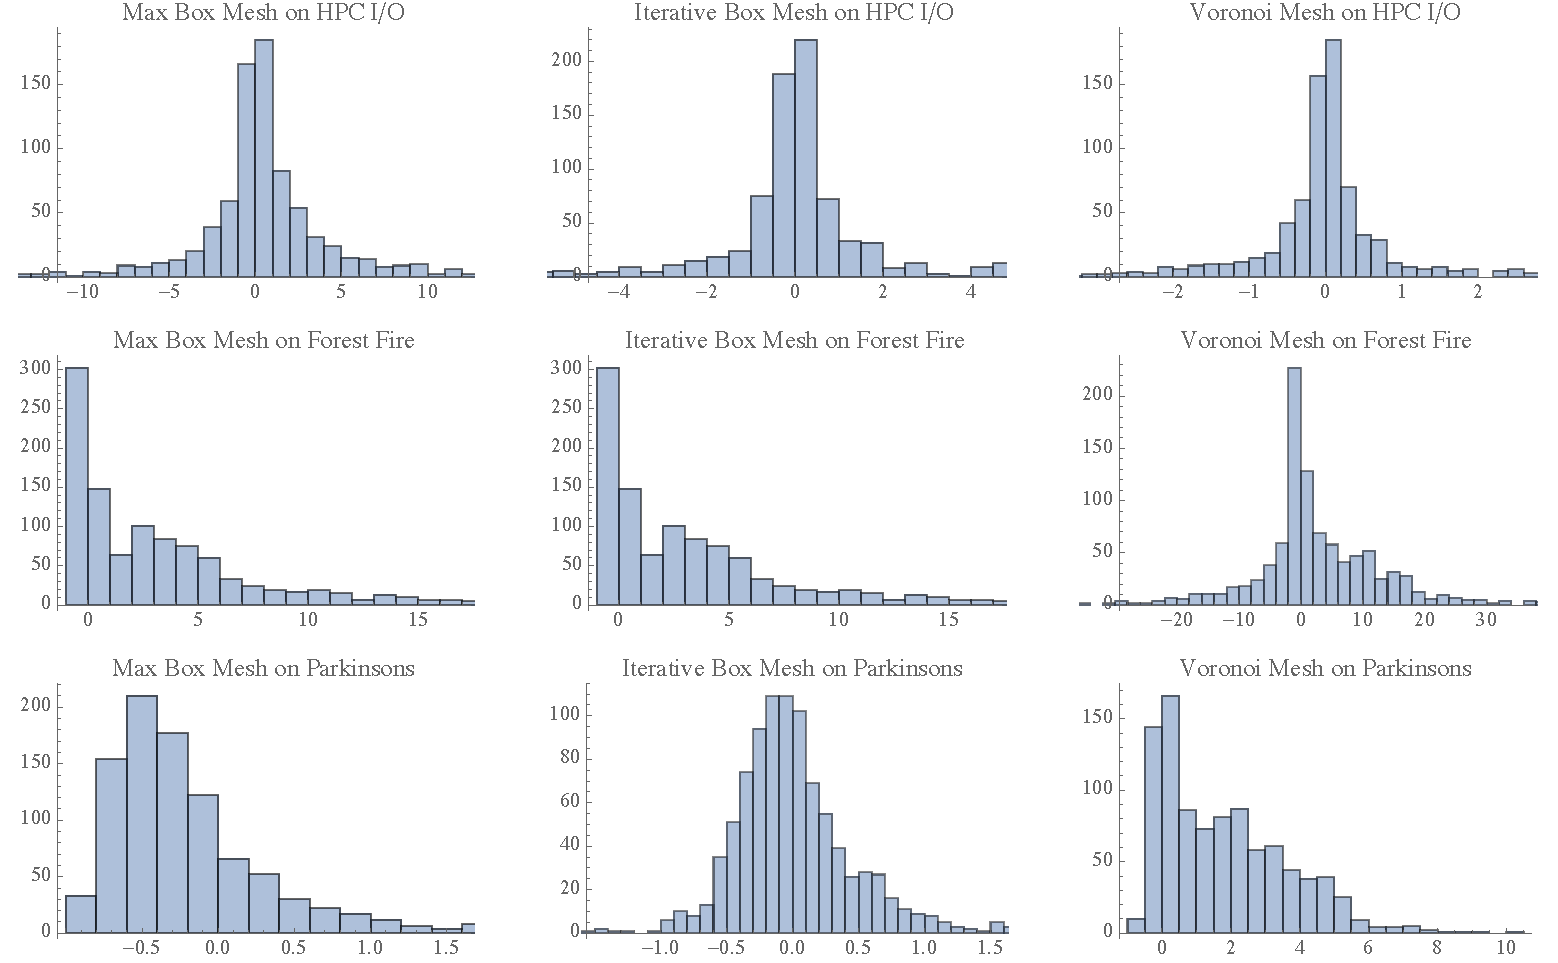
\includegraphics[width=0.95\textwidth,height=9.5cm]{perf-sample.pdf}};
    \node[below=of img, node distance=0cm, yshift=1cm] {Signed Relative Error in Prediction};
    \node[left=of img, node distance=0cm, rotate=90, anchor=center,yshift=-0.7cm] {Count};
  \end{tikzpicture}
  \caption{A sample of relative errors for all three techniques with optimal selections of error tolerance. The columns are for Max Box Mesh, Iterative Box Mesh, and Voronoi Mesh, respectively. The rows are for HPC I/O, Forest Fire, and Parkinsons respectively. Notice that the Max Box Mesh exibits the least skewed distribution of errors across all three data sets.
    \vspace{-.3cm}}
  \label{fig_perf_sample}
\end{figure*}

The selection of bootstrapping error tolerance also effects the computation time required to fit each of the models to data. Figure \ref{fig_eval_times} presents the time required to construct approximations for each model and each data set with varying $t$. The rapid reducting in computation time required for the forest fire and HPC I/O data sets suggests that large reductions in error can be achieved with relatively few basis functions. The Parkinson's data set however presents a more noisy response, with increasing number of basis functions reducing error much less quickly.

The distributions of errors experienced by each approximation technique when the optimal bootstrapping relative error tolerance is selected can be seen in Figure \ref{fig_perf_sample}. HPC I/O exibits the most normal approximation errors, which suggests that the models are converging on the latent noise of the response for the data set. The worst relative approximation errors are produced by the Voronoi mesh on the forest fire data set. The small magnitude true response values contribute to the larger relative errors, however the $VM$ performances are still unacceptably large.

\begin{figure*}
  \begin{tikzpicture}
    \node (img)  {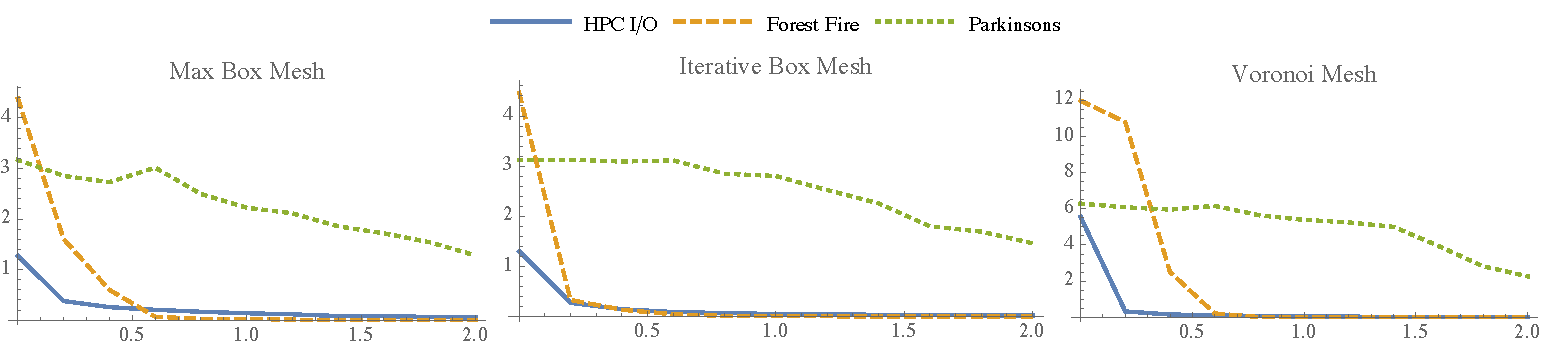
\includegraphics[width=0.95\textwidth,height=4cm]{eval-times.pdf}};
    \node[below=of img, node distance=0cm, yshift=1cm] {Relative Error Tolerance while Bootstrapping};
    \node[left=of img, node distance=0cm, rotate=90, anchor=center,yshift=-0.7cm] {Fit Time};
  \end{tikzpicture}
  \caption{Time required to generate model fits for each technique with varying relative error tolerance during bootstrapping.
    \vspace{-.3cm}}
  \label{fig_eval_times}
\end{figure*}

\section{Discussion}

The bootstrapping procdure presented for each approximation technique still has much room for improvement. Initial analysis suggests that the appropriate relative error tolerance needs to be discovered emperically for each application of a modelling technique. Further analytic studies could arrive at methods for determining optimal error tolerances at runtime, however increases in runtime complexity may not be afforded in many applications. 

The box-shaped basis functions and the construction algorithms used for the $MBM$ and $IBM$ could become a source of error when $d$ (the dimension of the data $X$) is much larger than $n$ (the number of known points). The blending regions in which multiple basis functions overlap are always axis aligned and in applications such as image analysis, any single dimension may be unsuitable for approximating the true underlying function. The Voronoi mesh attempts to address this problem by utilizing boundaries between points in multiple dimensions simultaneously. However, it is empirically unclear whether true benefits are seen in applications where $d < n$.

Each of the case studies presented have fewer than $1000$ points. The complexities of the presented approximation techniques are suitable for large dimension, but the increased complexity associated with brute-force bootstrapping currently prohibits their use on larger data sets. The Voronoi mesh in particular has a large complexity with respect to $n$ which could be significantly improved via more greedy bootstrapping. While each technique requires less than ten seconds on average to produce a fit in the presented case studies, the fit time required quickly grows into minutes around $1000$ points. While these initial results appear somewhat limiting, they demonstrate the viability of each mesh and leave room for further theoretical exploration of techniques to reduce the runtime complexity while maintaining the approximation power and flexibility.

\section{Conclusion}

The Max Box Mesh, Iterative Box Mesh, and Voronoi Mesh each provide novel strategies for effectively approximating multivariate phenomonon. The underlying constructions are theoretically straightforward, yet powerful and flexible. The computational complexities of each make them particularly suitable for applications in many dimensions, while the bootstrapping error tolerance parameter allows a balance between approximation and interplation to be explored empirically with each application.

\subsection{Future Work}

A thorough comparison with constituent multivariate approximation techniques including but not limited to, Linear Shepard interpolation, Multivariate Adaptive Regression Splines, Multi Layer Perceptron regression, and Delaunay Triangulation constitutes future work. A more detailed study of alternative bootstrapping techniques may also provide valuable insight.


\bibliographystyle{ACM-Reference-Format}
\bibliography{meshes} 

\end{document}
